\documentclass[a4paper]{article} %
\usepackage{graphicx,amssymb} %
%\usepackage[left=35mm, right=35mm, top=15mm, bottom=20mm, noheadfoot]{geometry}
\usepackage[utf8]{inputenc}
\usepackage{caption}
\usepackage{subcaption}
\graphicspath{{figuras/}}


\textwidth=15cm \hoffset=-1.2cm %
\textheight=25cm \voffset=-2cm %

\pagestyle{empty} %

\date{} %

%\def\keywords#1{\begin{center}{\bf Keywords}\\{#1}\end{center}} %
\def\keywords#1{{\bf Keywords: }{#1}}

% begin the document
\begin{document}
\thispagestyle{empty}

\title{\textbf{Title}}

% Authors
\author{Anderson A. Borba, \\ 
         PPGEEC - Programa de Pós-Graduação em Engenharia Elétrica e Computação\\
	 Universidade Presbiteriana Mackenzie\\
	 ISITEC - Instituto Superior de Inovação e Tecnologia\\
         São Paulo, Brasil\\ \\ % Affiliation 1
         Maurício Marengoni  \\ % If any other author with different Affilation
	 Universidade Presbiteriana Mackenzie\\
         São Paulo, Brasil \\ \\ % Affiliation 2 (if needed)
	% New author \\
	% New affiliation \\
	% Add authors and affiliation as needed
	\tt{anderborba@gmail.com} % Only one corresponding e-mail
}%

\date{} % <--- leave date empty
\maketitle\thispagestyle{empty} %% <-- you need this for the first page


\begin{abstract}
This paper presents a new kind of edge detector using the principal elements of  Multigrid edge detector methods.  The Multigrid methods are applied in partial differential equations (PDE's) and widely used in areas like engineering, physics, mathematics and computer science. The computational vision is a sub-area of computer science where the PDE is applieds for edge detection and image segmentation.

An efficient setup for edge detectors based on the caracteristics of the Multigrid methods is proposed, and it is shown the results of these operators applied on a set of imagens. A comparison  with methods well established in the literature is part of the analysis and results dissemination.

One of the methods proposed shown a better accuracy and noise reduction although the processing time was higher.
\end{abstract}

\keywords{Multigrid Methods, Computational Vision, Edge detection, Sobel operators, Laplacian methods.}

\section{Introdução}
Esta pesquisa apresenta a interação entre a ciência da computação através da área de visão computacional e a matemática aplicada. Os detectores de bordas baseados nos métodos Multigrid fazem a interação entre as áreas e potencializam suas características, ou seja, a fundamentação teórica da matemática aplicada tem potencial de suportar a proposição de um detector de borda. É destacado assim, a característica interdisciplinar da área de visão computacional.     
Os métodos  de resolução de sistemas lineares, entre eles o Multigrid tem se destacado, assim como sua implementação usando o paradigma de computação paralela. Sua  aplicabilidade  tem  sido em  sistemas lineares  provenientes  da discretização das Equações Diferenciais Parciais (EDP's). Outra idéia central é que os métodos Multigrid potencializam características dos métodos iterativos lineares. Por este motivo, quando aplicados em EDP's, com aumento ou redução da resolução, intensificamos suas características como a independência ao refinamento, ótimo controle de ruído e escalabilidade com algoritmos paralelos.

Devido ao conhecimento das características salientadas são propostos dois novos detectores de bordas baseados nos métodos Multigrid aplicados em visão computacional. Vamos chamar estes detectores de bordas como Operador Laplaciano Multigrid (OLM) e Operador Laplaciano Multigrid Modificado (OLMM).


No contexto histórico os primeiros  estudos  investigando  os  métodos Multigrid  foram  feitos  por Fedorenko \cite{Fedorenko1962relaxation,Fedorenko1964speed} entre $1962$ e $1964$, e Bakhvalov \cite{Bakhvalov} em $1966$. Tanto Fedorenko quanto Bakhvalov investigaram a  convergência dos problemas de valor com fronteira de segunda ordem. Entre  $1975$ e $1976$ Hackbusch \cite{Hackbusch1980convergence} desenvolveu os  elementos fundamentais  dos métodos Multigrid,  trabalhando com  investigações  teóricas  e aplicações práticas dos métodos.

Um artigo clássico e de grande importância para os métodos Multigrid é o trabalho de Brandt \cite{brandt1977multi}  que reúne ideias desenvolvidas de $1970$  até $1977$. Neste  artigo Brandt investiga  sobre  os métodos  lineares e não lineares,  técnicas adaptativas  aplicadas, malhas não uniformes, experimentos numéricos para EDP's usando o método Multigrid.


As ideias investigadas neste artigo foram baseadas em estudos prévios dos autores e nos artigos de Perona e Malik \cite{perona1990scale}, Scott \cite{scott1998multigrid}, Papandreou e Maragos \cite{papandreou2007multigrid}, Tisotdios e Petrou \cite{tsiotsios2013anisotropic}. O tema que envolve detecção de borda nas áreas de visão computacional e processamento de imagens é atual e desafiador, como podemos constatar nos artigos de Liu et al \cite{liu2017multigrid} e  Molina et al \cite{molina2014impact}. O artigo de Molina et al \cite{molina2014impact} mostra o estudo das equações diferenciais anisotrópicas para detecção de borda e a importância de resolver eficientemente estas equações. Quanto ao artigo de Liu\cite{liu2017multigrid} aparece EDP's isotrópicas tridimensionais aplicadas em imagens médicas, o que mostra a necessidade da criação de um método que conecte Multigrid  e detecção de borda de forma a produzir um método eficiente e consistente.

No contexto acima podemos notar a importância do estudo de equações anisotrópicas somado ao tratamento das equações quando o domínio é tridimensional, salientando que equações tridimensionais são tratadas de maneira isotrópicas. Desta forma, os dois últimos artigos mostram que pesquisar o tema detectores de bordas, em equações anisotrópicas, e sua natural evolução para o domínio tridimensional fazem parte do estado da arte na área de visão computacional e matemática aplicada.   
Para melhor descrever o tema proposto, o presente trabalho está dividido da seguinte maneira: uma introdução mostrando o contexto histórico dos métodos, posteriormente na seção $(II)$ a descrição dos métodos com suas principais referências. Na seção $(III)$ podemos ver as imagens geradas pelos métodos e as análises das características dos métodos propostos com intuito de validar sua aplicação e principalmente sintonizar os componentes independentes dos operadores (filtros). No fim deste artigo, seção $(IV)$, os autores apresentam conclusões e possibilidades de futuras pesquisas. 

\section{Descrição dos métodos}
Nesta seção serão descritos os operadores que aplicamos na presente pesquisa. Uma referência que faz uma revisão das últimas duas décadas de publicações sobre detecção de bordas pode ser encontrada em Oskoei e Hu \cite{oskoei2010survey}.
\subsection{Operador de Sobel.}

O operador de Sobel, ou filtro de  Sobel é usado em processamento de imagens e visão computacional, mais especificamente na área de detecção de borda.

 Este operador surgiu no artigo de Sobel e Feldman \cite{sobel1968}. O operador consiste em uma aproximação discreta do operador de diferenciação para o gradiente de uma imagem.                 


O operador de Sobel usa dois núcleos que são convoluídos com a imagem original para gerar uma aproximação do gradiente da imagem. Sendo a imagem $I(x, y)$ podemos definir os núcleos $G_x$ e $G_y$. Ou seja, o primeiro operador (núcleo) armazena a aproximação na direção de $x$ e o segundo operador (núcleo) armazena a aproximação na direção $y$. Para maiores detalhes pode-se consultar o artigo original de Sobel e Feldman, já citado, ou o artigo de Gupta e Mazumdar \cite{gupta2013sobel}.  

%\begin{equation}
% I_{i,j}^{t+1} = a_eI_{i+1,j}^{t}+a_wI_{i-1,j}^{t}+a_cI_{i,j}^{t}+a_nI_{i,j+1}^{t}+a_sI_{i,j-1},\label{equa1:2}
%\end{equation}

$$G_x* I(x,y)=\left[
\begin{array}{lll}
-1 & 0 & 1\\
-2 & 0 & 2\\
-1 & 0 & 1\\
\end{array}
\right]_{3 \times 3}* I(x,y).$$

$$G_y* I(x,y)=\left[
\begin{array}{rrr}
 1 &  2 &  1\\
 0 &  0 &  0\\
-1 & -2 & -1\\
\end{array}
\right]_{3 \times 3}* I(x,y).$$

Os principais passos da implementação do operador de Sobel são mostrados abaixo.

\begin{description}
\item[(1)] Aplicar um borrador (filtro) Gaussiano na imagem.
\item[(2)] Aplicar o Sobel ($G_x$) na imagem.
\item[(3)] Aplicar o Sobel ($G_y$) na imagem.
\item[(4)] Ponderar $G_x$ com $G_y$ aplicados na imagem.
\end{description}

Os parâmetros definidos na programação dos operadores utilizados neste estudo seguem o padrão da biblioteca  OpenCV \cite{opencv_3_2016} usados juntamente com a linguagem C \cite{ling_c}.

\subsection{Operador $LoG$ - Laplaciano da Gaussiana.}

Filtros Gaussianos são amplamente usados em processamento  de imagens e detecção de bordas. Os pioneiros que proporam um detector de borda baseado em filtros Gaussinos foram Marr e Hildreth \cite{marr1980theory}.

O método consiste em aplicar um borrador (filtro) Gaussiano na imagem e posteriormente usar o núcleo gerado pela aproximação discreta do Laplaciano que pode ser representado por: 
$$L* G(I(x,y))=\left[
\begin{array}{lrl}
 0 &  1 & 0\\
 1 & -4 & 1\\
 0 &  1 & 0\\
\end{array}
\right]_{3 \times 3}* G(I(x,y)),$$
sendo $G(I(x,y))$ a função Gaussiana aplicada na imagem.

Os principais passos da implementação do operador $LoG$ são mostrados abaixo.

\begin{description}
\item[(1)] Aplicar um borrador (filtro) Gaussiano na imagem.
\item[(2)] Aplicar o operador Laplaciano no resultado de $(1)$.
\end{description}

Para melhor entendimento das características do método, o relatório técnico de Oskoei e Hu \cite{oskoei2010survey} apontam pontos fortes e fracos do operador $LoG$.


\subsection{Operador com Multirresolução ou $LoG$ Piramidal.}


Um artigo pioneiro na área foi escrito por Schunck \cite{schunck1987scale}. Esse método repete o método anterior até o segundo passo, logo após temos a aplicação da teoria de imagem piramidal, que consiste em sucessivas aplicações de operadores de restrição até uma imagem com resolução de referência, e posterior aplicação do operador de interpolação até a resolução da imagem de entrada. 

Os principais passos da implementação do operador $LoG$ Piramidal são mostrados abaixo.

\begin{description}
\item[(1)] Aplicar um borrador (filtro) Gaussiano  na imagem.
\item[(2)] Aplicar o operador Laplaciano no resultado de $(1)$.
\item[(3)] Aplicar os operadores de restrição.
\item[(4)] Aplicar os operadores de interpolação.
\end{description}


\subsection{Operador Laplaciano Multigrid (OLM).}

As referências teóricas para o problema na área de visão computacional são encontradas e descritas nas seguintes referências, Perona \cite{perona1990scale}, Papandreou \cite{papandreou2007multigrid}, Tsiotsios \cite{tsiotsios2013anisotropic}. A equação
%{\bf PROBLEMA MODELO }
\begin{equation}\label{eq1}
\left\{\begin{array}{lc}
I_t=div(c(x,y,t)\nabla I), & \forall x,y\in \Omega\\
I(x,y,t)=g, & \forall x,y\in\partial{\Omega}\\
I(x,y,t_0)=I_0(x,y,0), & \forall x,y\in \Omega
\end{array}
\right.
\end{equation}

é uma equação diferencial parcial (EDP) evolutiva, conhecida como equação de difusão anisotrópica. Maiores detalhes sobre a anisotropia, condições iniciais e fronteira estão descritos em Perona e Malik \cite{perona1990scale}.

A discretização da EDP é realizada por diferenças finitas com aproximação de segunda ordem. O artigo de Perona e Malik \cite{perona1990scale} estabelece com propriedade as questões envolvidas na discretização desta EDP. Aplicando-se essas ideias geramos a seguinte equação de diferenças
\begin{equation}\label{eq2}
 I_{i,j}^{t+1} = a_eI_{i+1,j}^{t}+a_wI_{i-1,j}^{t}+a_cI_{i,j}^{t}+a_nI_{i,j+1}^{t}+a_sI_{i,j-1}^{t},
\end{equation}
sendo $a_e,a_w,a_c,a_n,$ e $a_s$ coeficientes da equação discreta de difusão anisotrópica. Na detecção de borda podemos desconsiderar a evolução temporal, resultando na seguinte equação de diferenças  
\begin{equation}\label{eq3}
0 = a_eI_{i+1,j}+a_wI_{i-1,j}+a_cI_{i,j}+a_nI_{i,j+1}+a_sI_{i,j-1},
\end{equation}

que pode ser representada pelo seguinte núcleo:
$$L* G(I(x,y))=\left[
\begin{array}{lrl}
 0 &  a_n & 0\\
 a_w &  a_c & a_e\\
 0 &  a_s & 0\\
\end{array}
\right]_{3 \times 3}* G(I(x,y)),$$
sendo $G(I(x,y))$ a função Gaussiana aplicada na imagem.

Baseado no operador com multirresolução e no conhecimento dos autores da teoria dos métodos Multigrid e visão computacional, propomos, neste artigo, dois detectores de bordas aos quais chamamos de Operador Laplaciano Multigrid (OLM) e Operador Laplaciano Multigrid Modificado (OLMM). Os operadores serão descritos nesta seção e na próxima, respectivamente. 

O método (OLM) consiste em aplicar a função Gaussiana na imagem e posteriormente usar o núcleo gerado pela aproximação discreta do Laplaciano, em cada nível de resolução. De maneira geral estamos aplicando o operador $LoG$ em cada nível de resolução de imagem, tanto na descida com o operador de restrição, como na subida com o operador de interpolação. 

Os principais passos do (OLM) são descritos da seguinte maneira:
\begin{description}
\item[(*)] Para cada nível de resolução faça.
\item[(1)] Aplicar um borrador (filtro) Gaussiano na imagem.
\item[(2)] Aplicar o operador Laplaciano  no resultado de $(1)$.
\item[(3)] Aplicar os operadores de restrição em $(2)$.
\item[(4)] Aplicar os operadores de interpolação $(3)$.
\item[(5)] Aplicar um borrador (filtro) Gaussiano na imagem após o passo $(4)$.
\item[(6)] Aplicar o Laplaciano  no resultado de $(5)$.
\end{description}

\subsection{Operador Laplaciano Multigrid Modifidado (OLMM).}

Este operador é baseado no operador Laplaciano Multigrid, porém, é proposto a supressão da aplicação do operador Gaussiano e Laplaciano após o processo de interpolação. A supressão foi realizada depois de uma análise da aplicação do operador (OLM), na próxima seção será enfatizado o motivo dessa modificação. 

Os principais passos do (OLMM) são descritos da seguinte maneira:
\begin{description}
\item[(*)] Para cada nível de resolução faça.
\item[(1)] Aplicar um borrador (filtro) Gaussiano na imagem.
\item[(2)] Aplicar o Laplaciano  no resultado de $(1)$.
\item[(3)] Aplicar os operadores de restrição em $(2)$.
\item[(4)] Aplicar os operadores de interpolação em $(3)$.
\end{description}


\section{Análise dos Métodos.}

\begin{figure}[!htb]
\minipage{0.32\textwidth}
  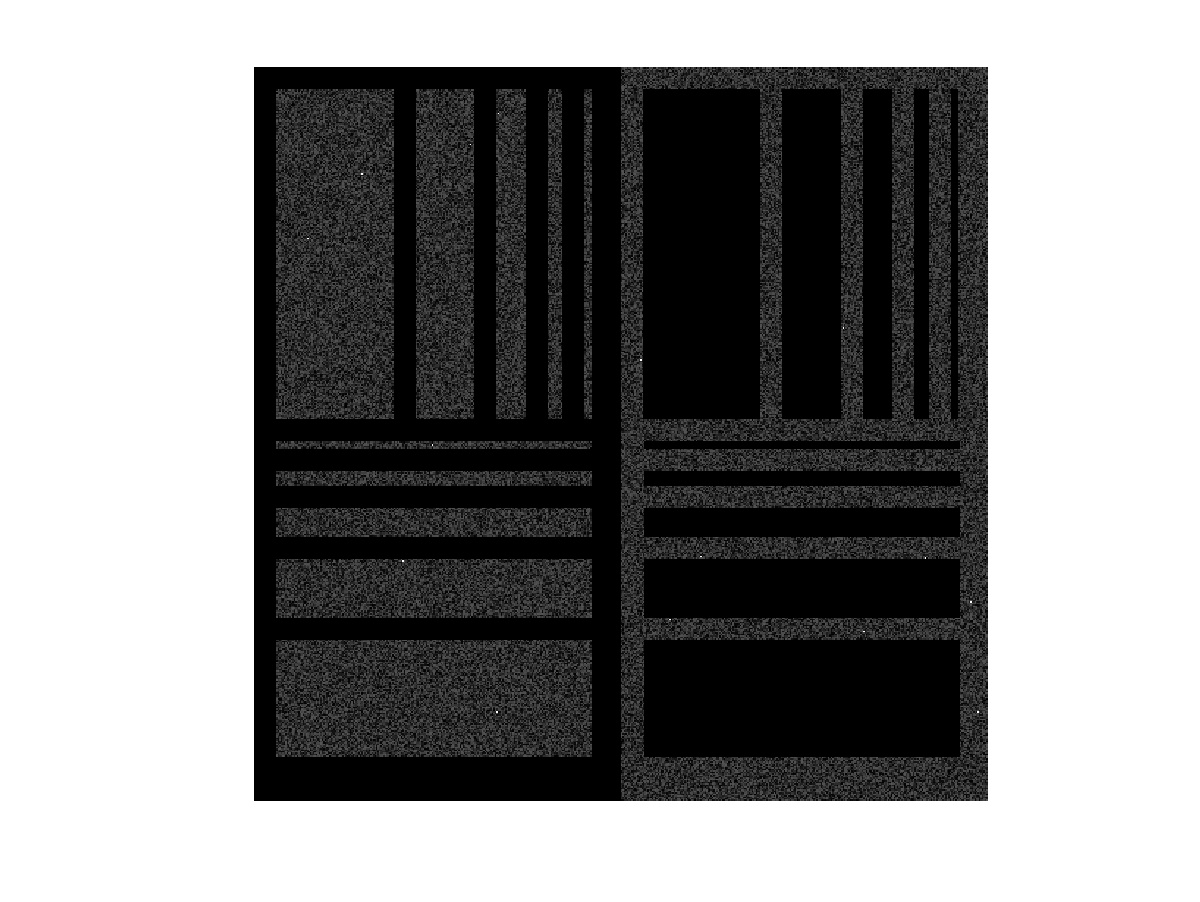
\includegraphics[width=\linewidth]{Eq_Phantom_0p000_4_1_1.jpg}
	\caption{Phantom $P_{1,4,0.0}$}\label{fig:awesome_image1}
\endminipage\hfill
\minipage{0.32\textwidth}
  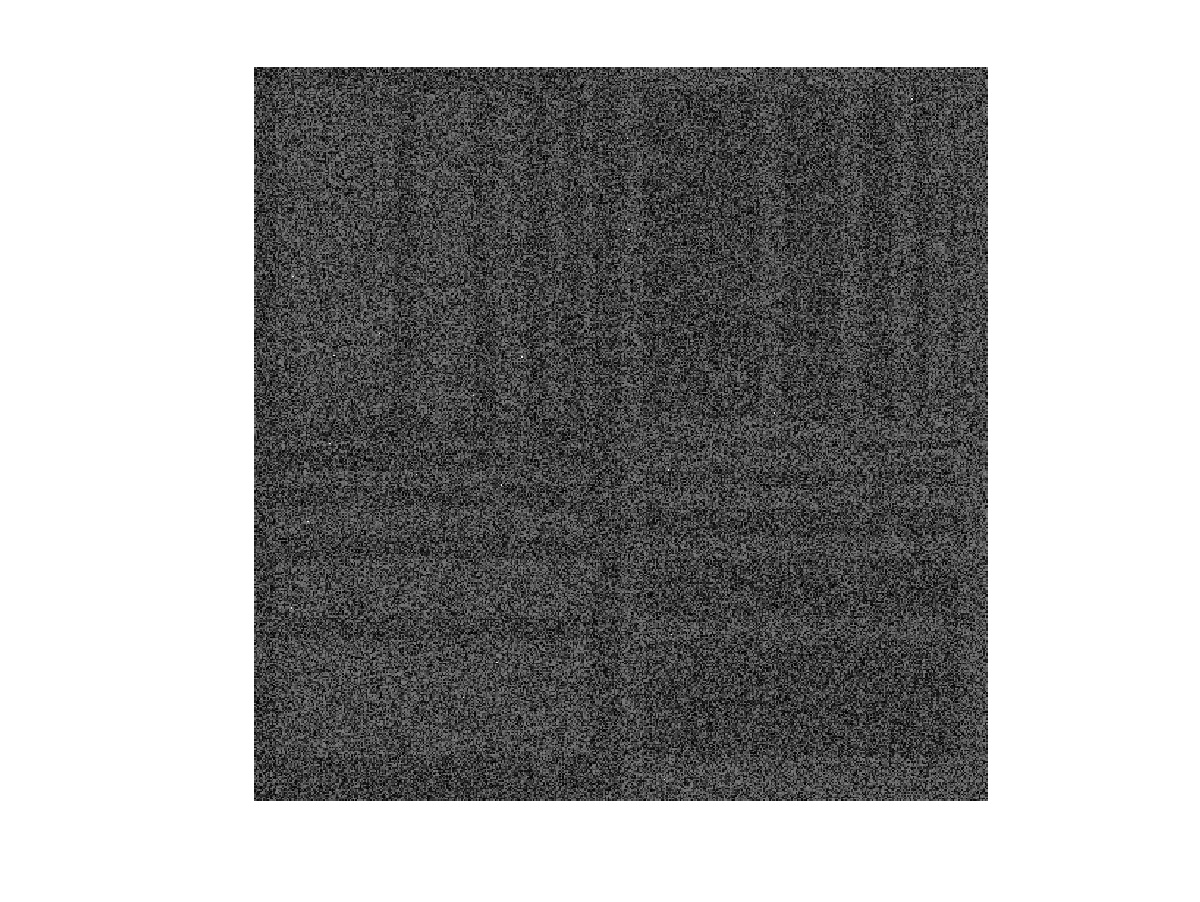
\includegraphics[width=\linewidth]{Eq_Phantom_0p500_4_1_1.jpg}
	\caption{Phantom $P_{1,4,0.5}$}\label{fig:awesome_image1}
\endminipage\hfill
\minipage{0.32\textwidth}%
  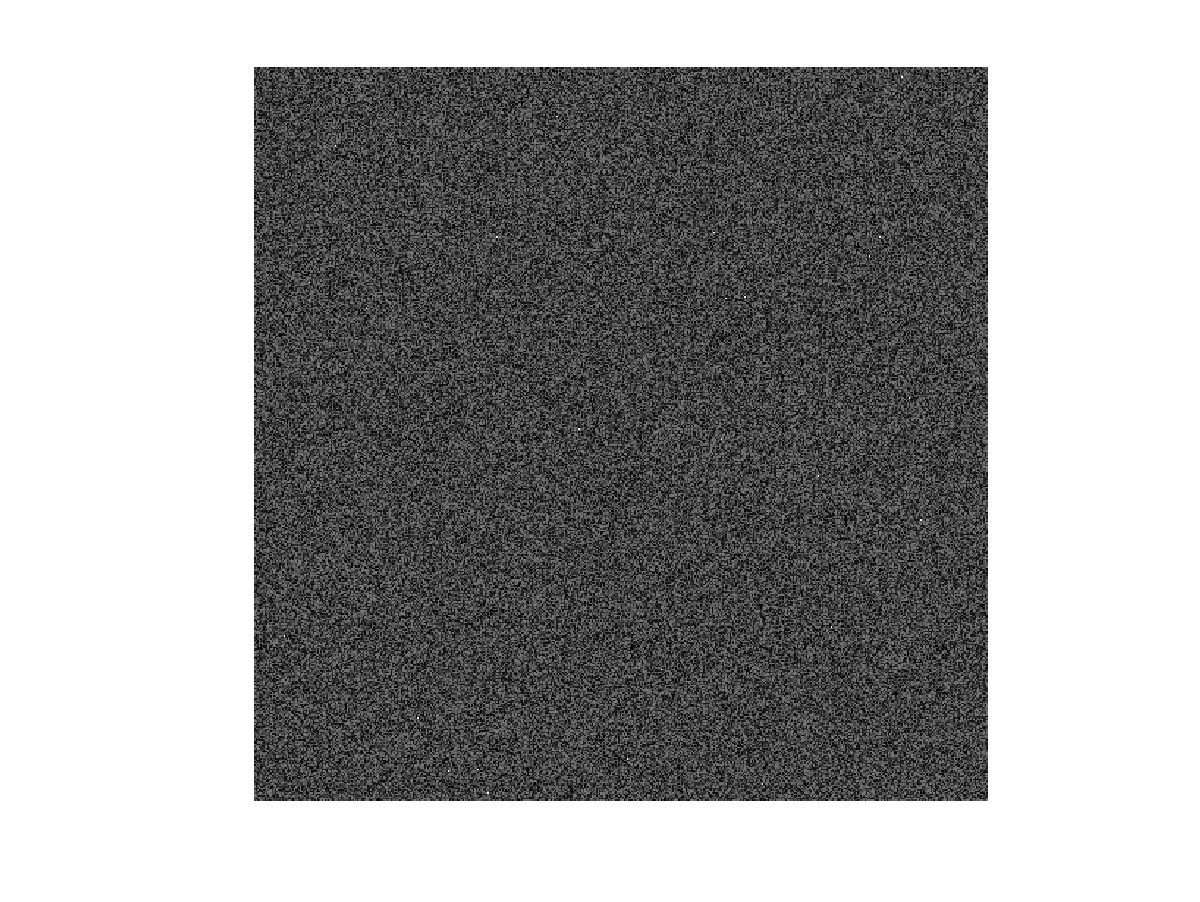
\includegraphics[width=\linewidth]{Eq_Phantom_0p700_4_1_1.jpg}
	\caption{Phantom $P_{1,4,0.7}$}\label{fig:awesome_image1}
\endminipage
\caption{A really Awesome Image}\label{fig:awesome_image3}
\end{figure}

\begin{figure}[!htb]
\minipage{0.20\textwidth}
  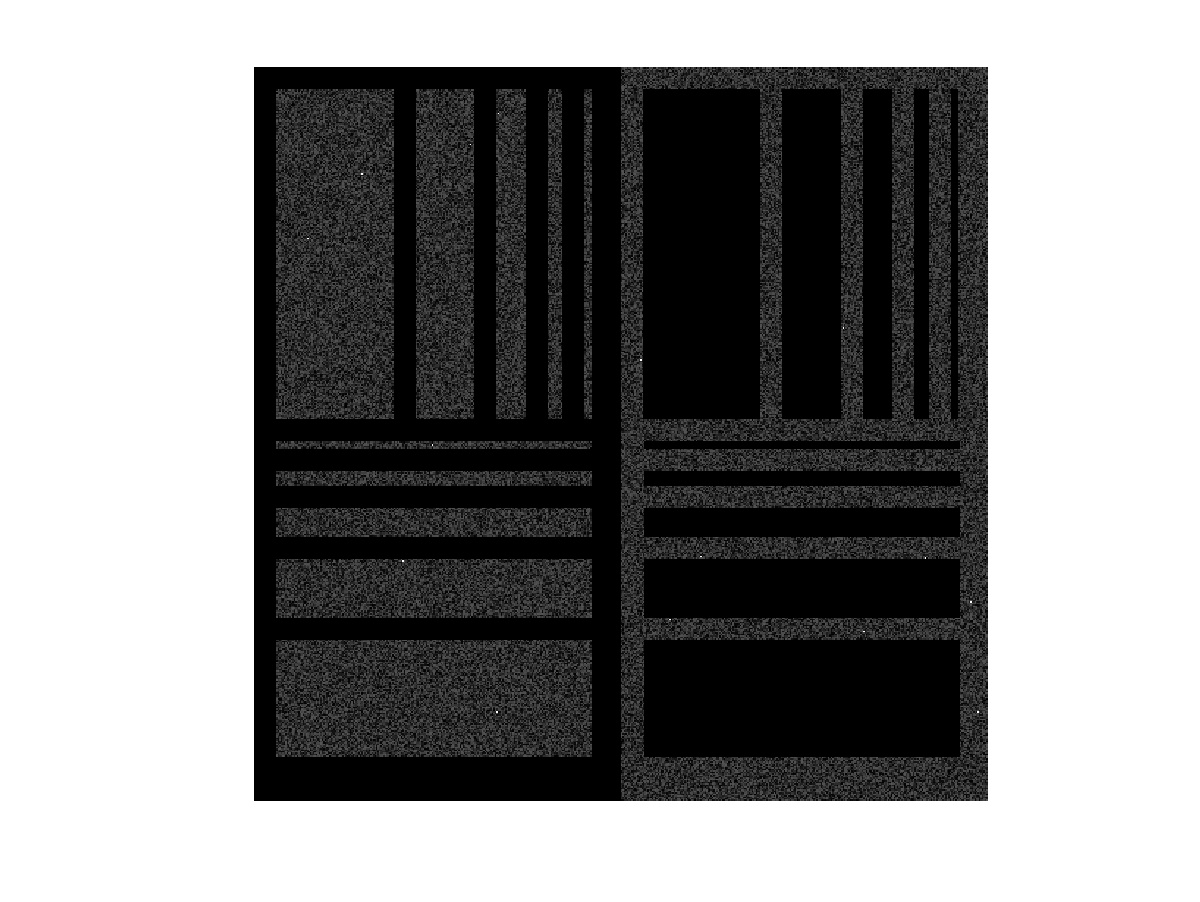
\includegraphics[width=\linewidth]{Eq_Phantom_0p000_4_1_1.jpg}
	%\caption{Phantom $P_{1,4,0.0}$}\label{fig:awesome_image1}
\endminipage\hfill
\minipage{0.20\textwidth}
  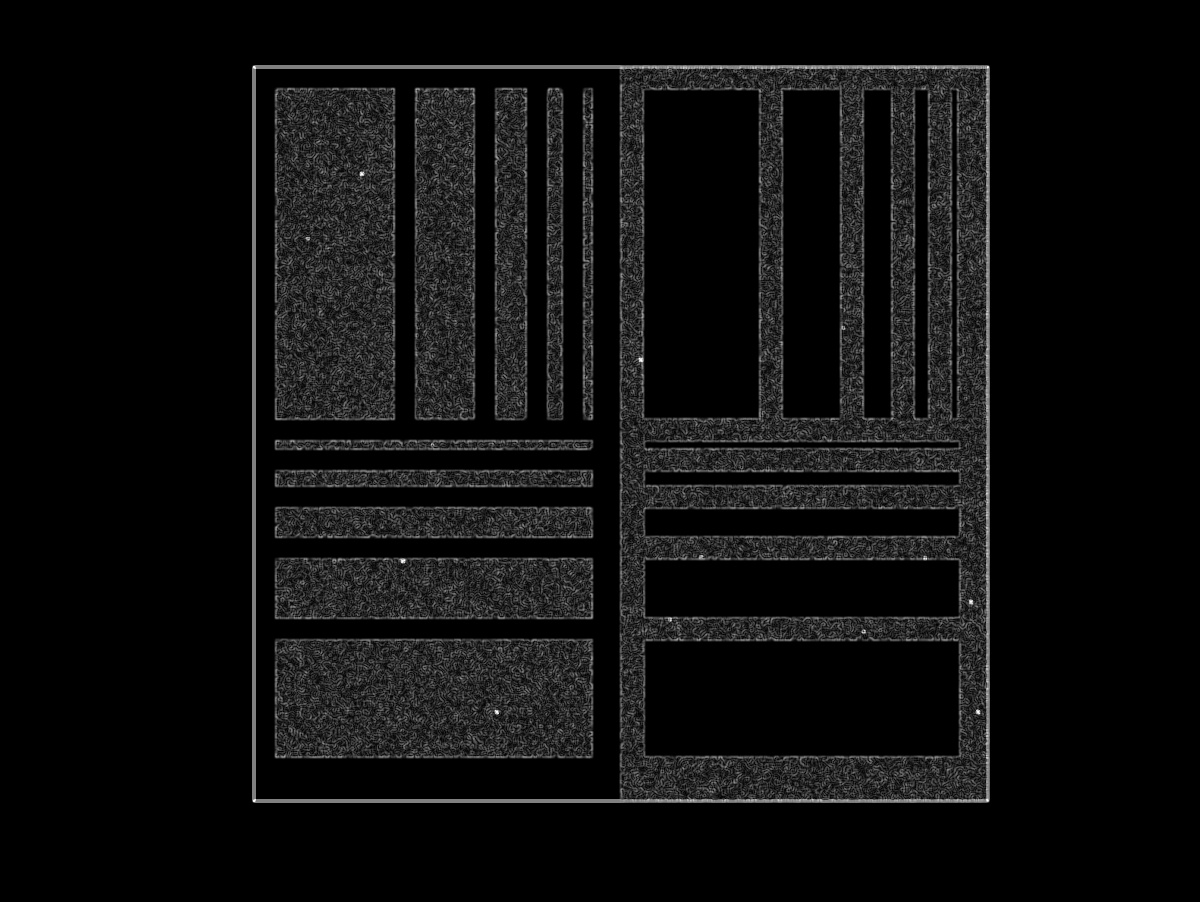
\includegraphics[width=\linewidth]{sobel_Eq_Phantom_0p000_4_1_1.jpg}
%  \caption{Sobel}\label{fig:awesome_image2}
\endminipage\hfill
\minipage{0.20\textwidth}%
  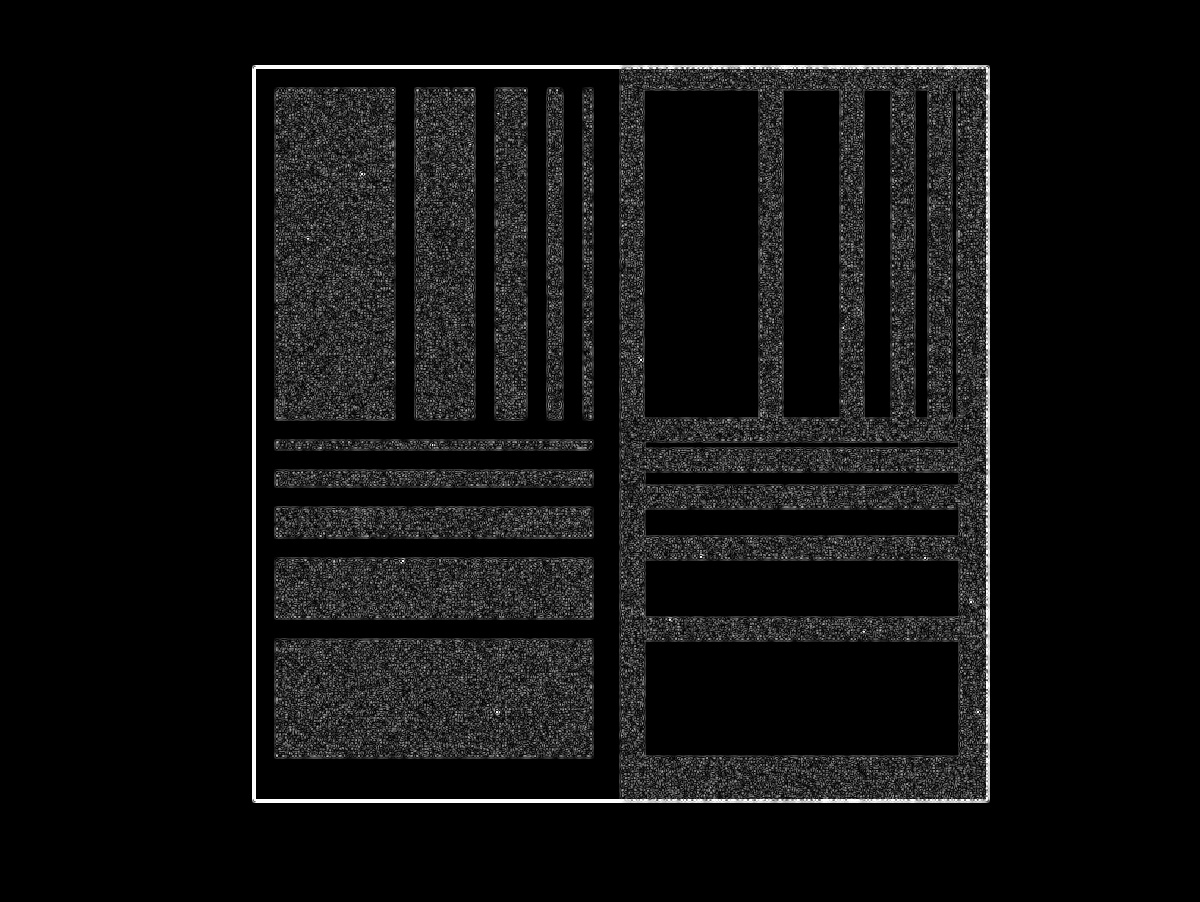
\includegraphics[width=\linewidth]{lap_Eq_Phantom_0p000_4_1_1.jpg}
%  \caption{Laplaciano}\label{fig:awesome_image3}
\endminipage\hfill
\minipage{0.20\textwidth}%
  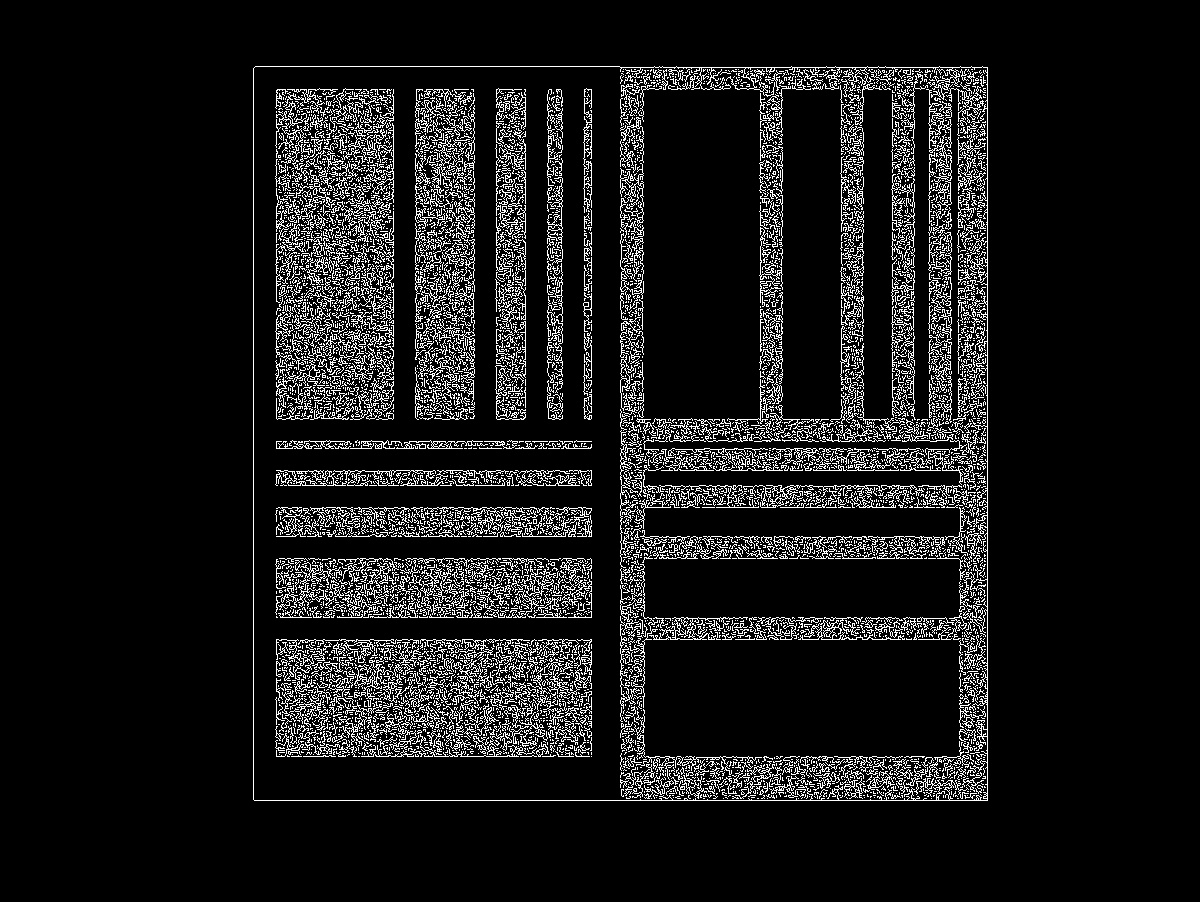
\includegraphics[width=\linewidth]{canny_Eq_Phantom_0p000_4_1_1.jpg}
%  \caption{Canny}\label{fig:awesome_image3}
\endminipage\hfill
\minipage{0.20\textwidth}%
  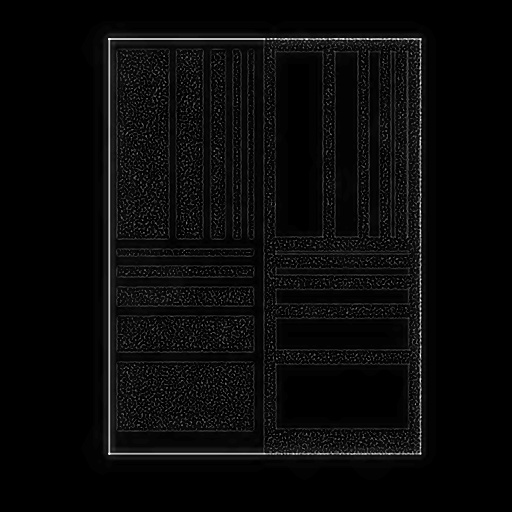
\includegraphics[width=\linewidth]{mult_Eq_Phantom_0p000_4_1_1.jpg}
%	\caption{Multigrid(Piramidal)}\label{fig:awesome_image3}
\endminipage\hfill
%%%%% Segunda linha
\minipage{0.20\textwidth}
  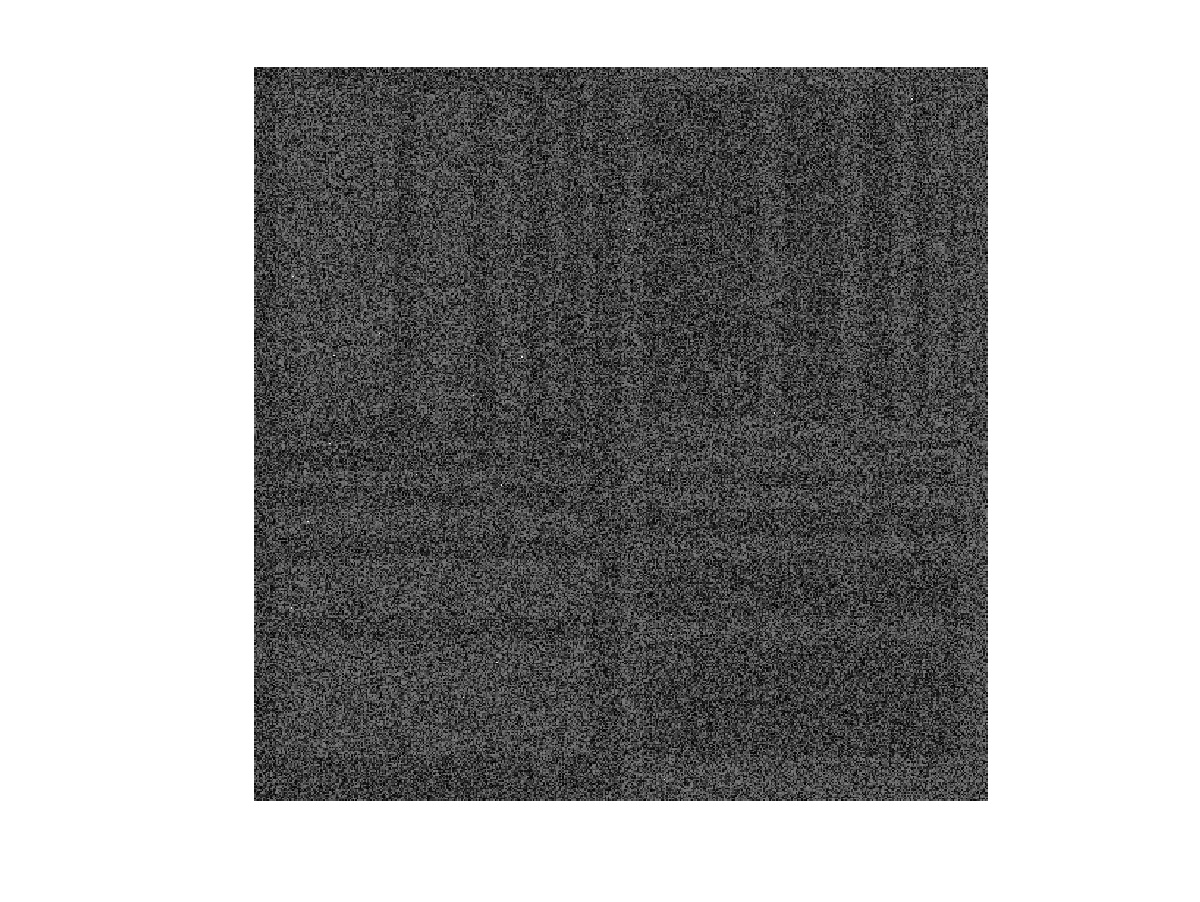
\includegraphics[width=\linewidth]{Eq_Phantom_0p500_4_1_1.jpg}
%	\caption{Phantom $P_{1,4,0.5}$}\label{fig:awesome_image1}
\endminipage\hfill
\minipage{0.20\textwidth}%
  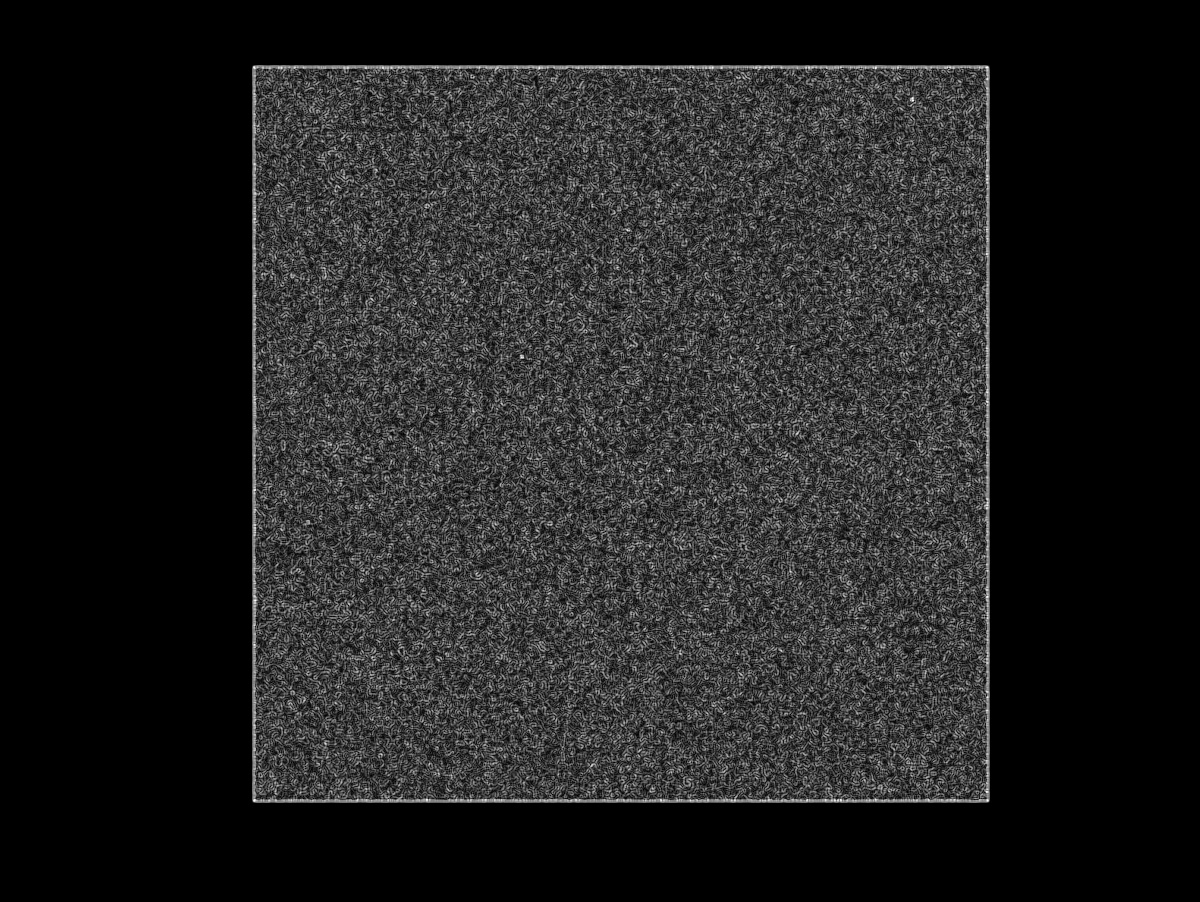
\includegraphics[width=\linewidth]{sobel_Eq_Phantom_0p500_4_1_1.jpg}
%  \caption{Sobel}\label{fig:awesome_image3}
\endminipage\hfill
\minipage{0.20\textwidth}%
  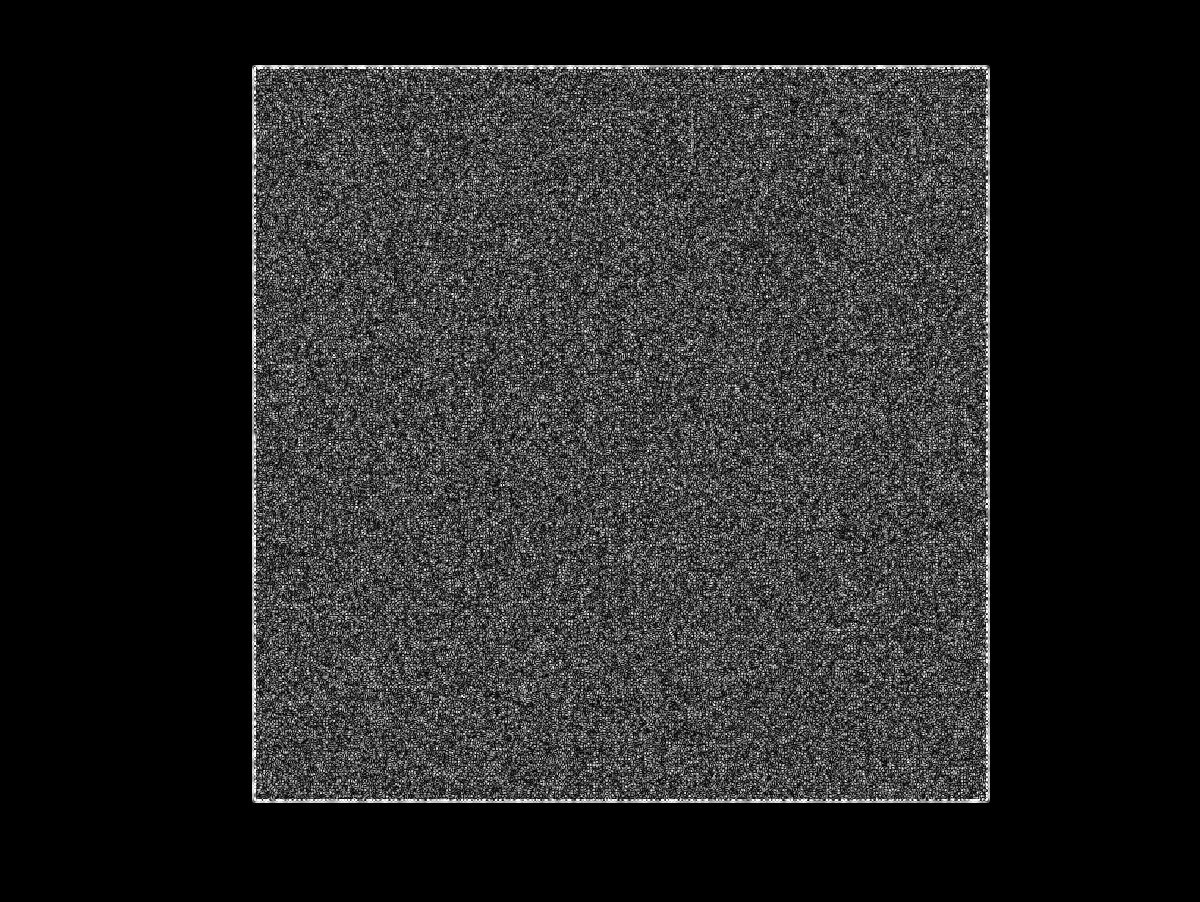
\includegraphics[width=\linewidth]{lap_Eq_Phantom_0p500_4_1_1.jpg}
%  \caption{Laplaciano}\label{fig:awesome_image3}
\endminipage\hfill
\minipage{0.20\textwidth}%
  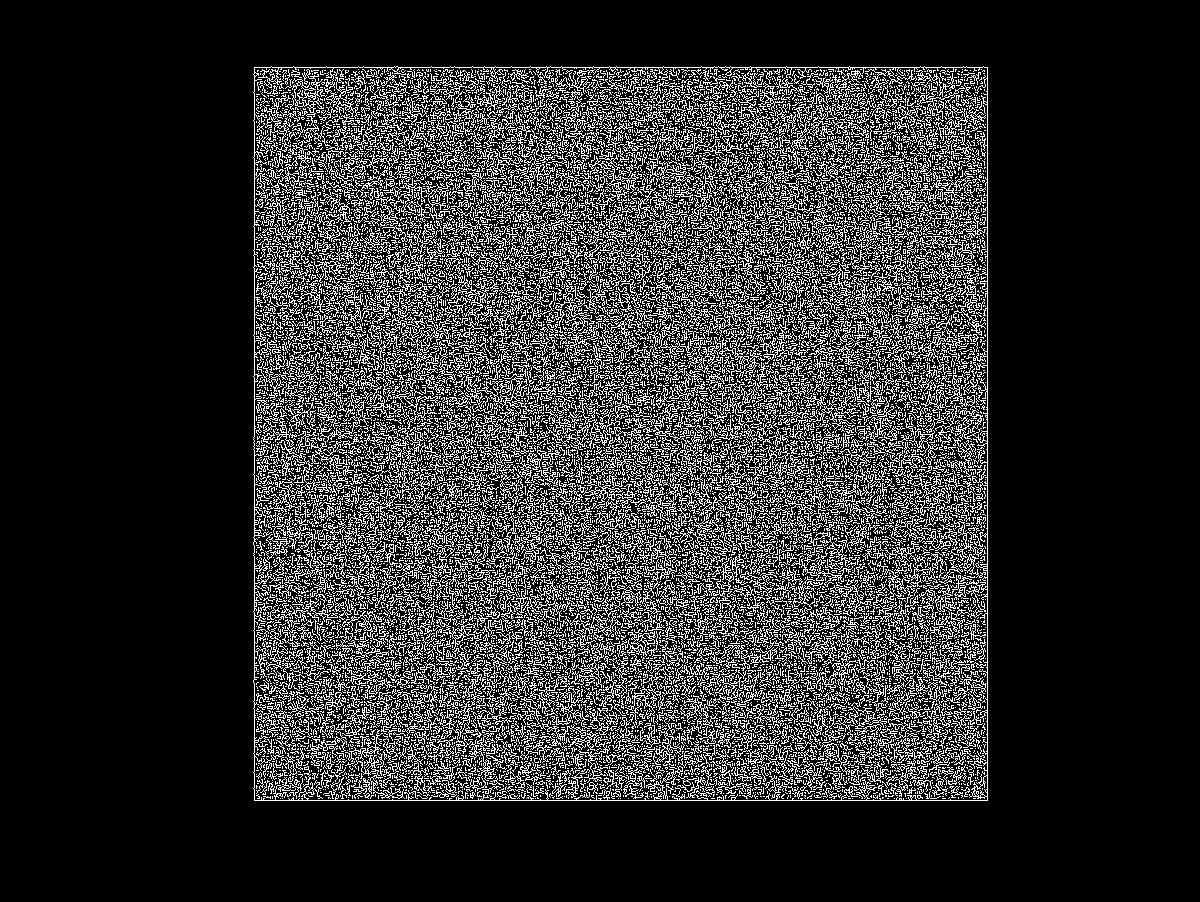
\includegraphics[width=\linewidth]{canny_Eq_Phantom_0p500_4_1_1.jpg}
%  \caption{Canny}\label{fig:awesome_image3}
\endminipage\hfill
\minipage{0.20\textwidth}%
  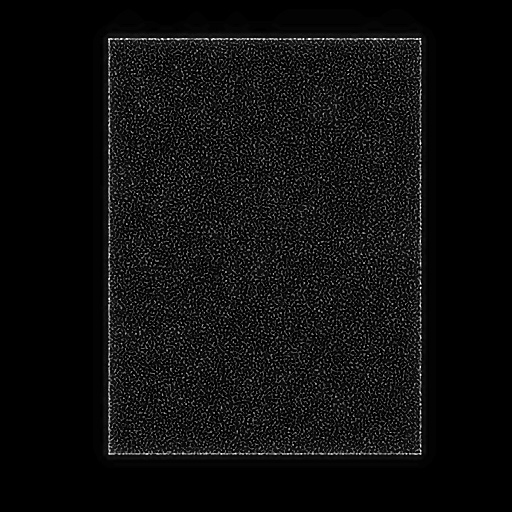
\includegraphics[width=\linewidth]{mult_Eq_Phantom_0p500_4_1_1.jpg}
%	\caption{Multigrid(Piramidal)}\label{fig:awesome_image3}
\endminipage\hfill
%%%%% Terceira  linha
\minipage{0.20\textwidth}
  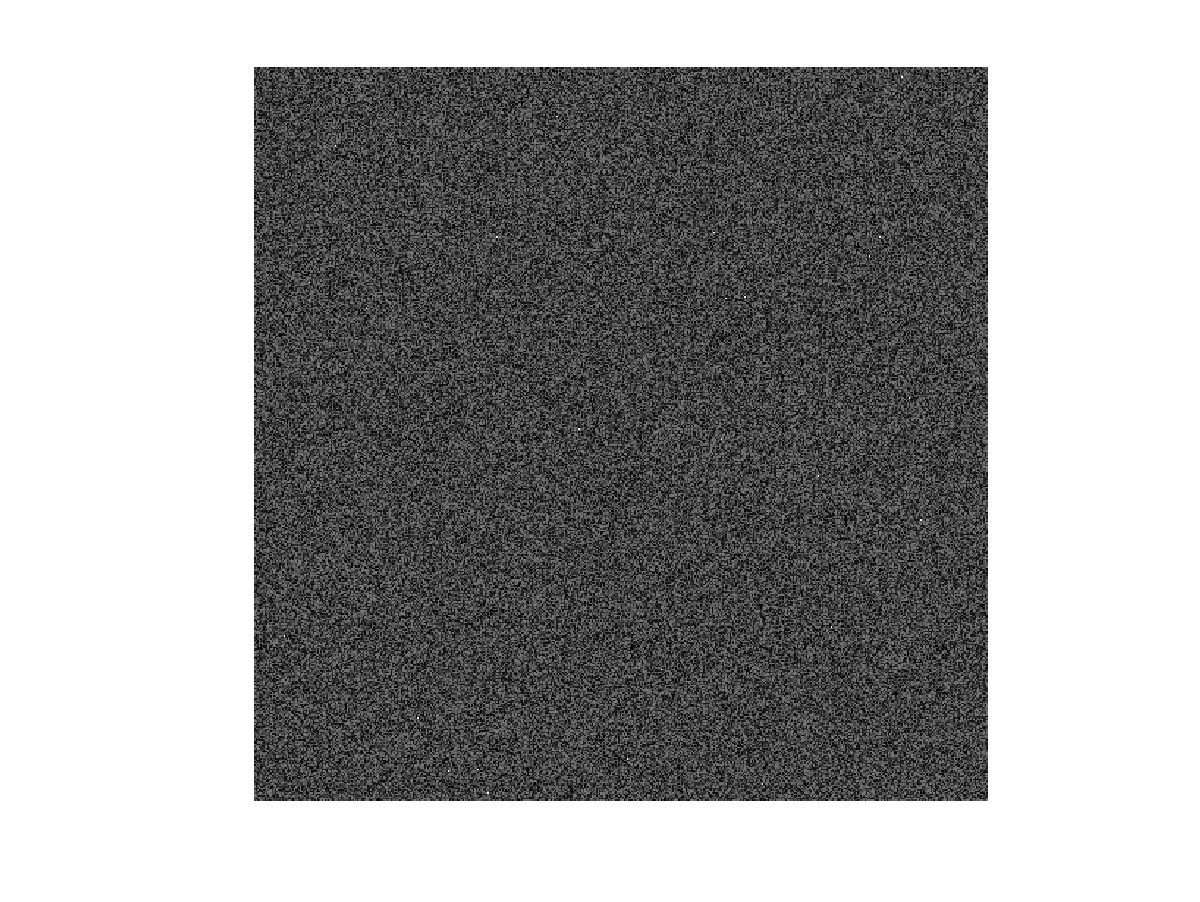
\includegraphics[width=\linewidth]{Eq_Phantom_0p700_4_1_1.jpg}
%	\caption{Phantom $P_{1,4,0.7}$}\label{fig:awesome_image1}
\endminipage\hfill
\minipage{0.20\textwidth}%
  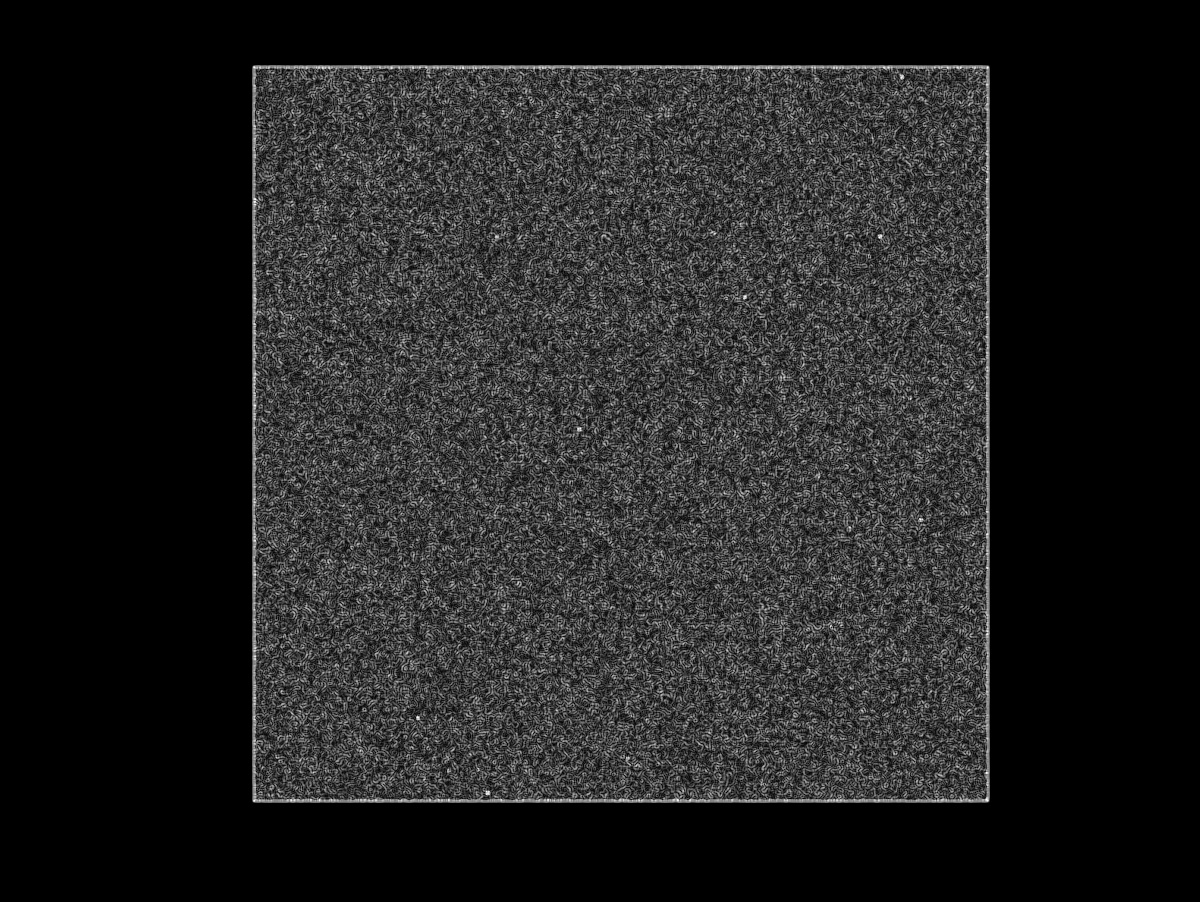
\includegraphics[width=\linewidth]{sobel_Eq_Phantom_0p700_4_1_1.jpg}
%  \caption{Sobel}\label{fig:awesome_image3}
\endminipage\hfill
\minipage{0.20\textwidth}%
  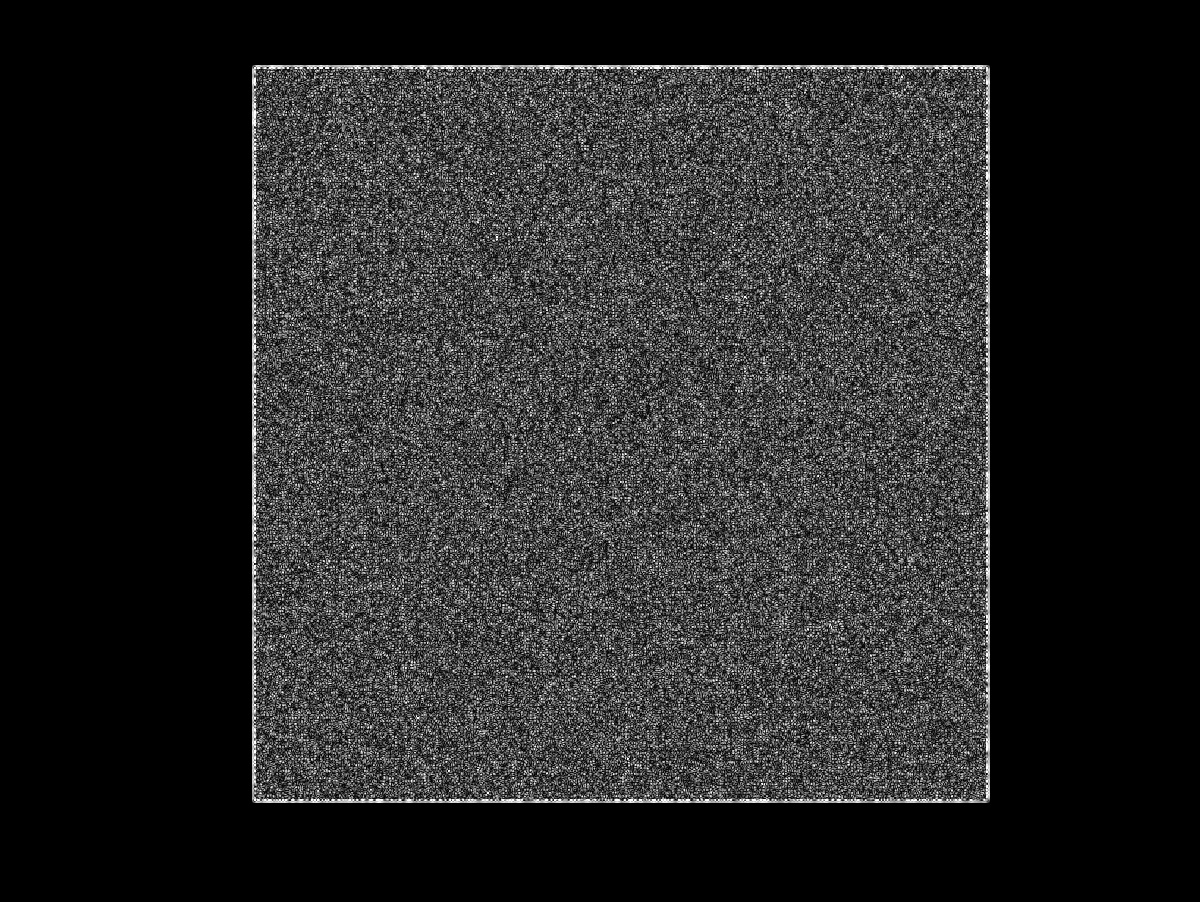
\includegraphics[width=\linewidth]{lap_Eq_Phantom_0p700_4_1_1.jpg}
%  \caption{Laplaciano}\label{fig:awesome_image3}
\endminipage\hfill
\minipage{0.20\textwidth}%
  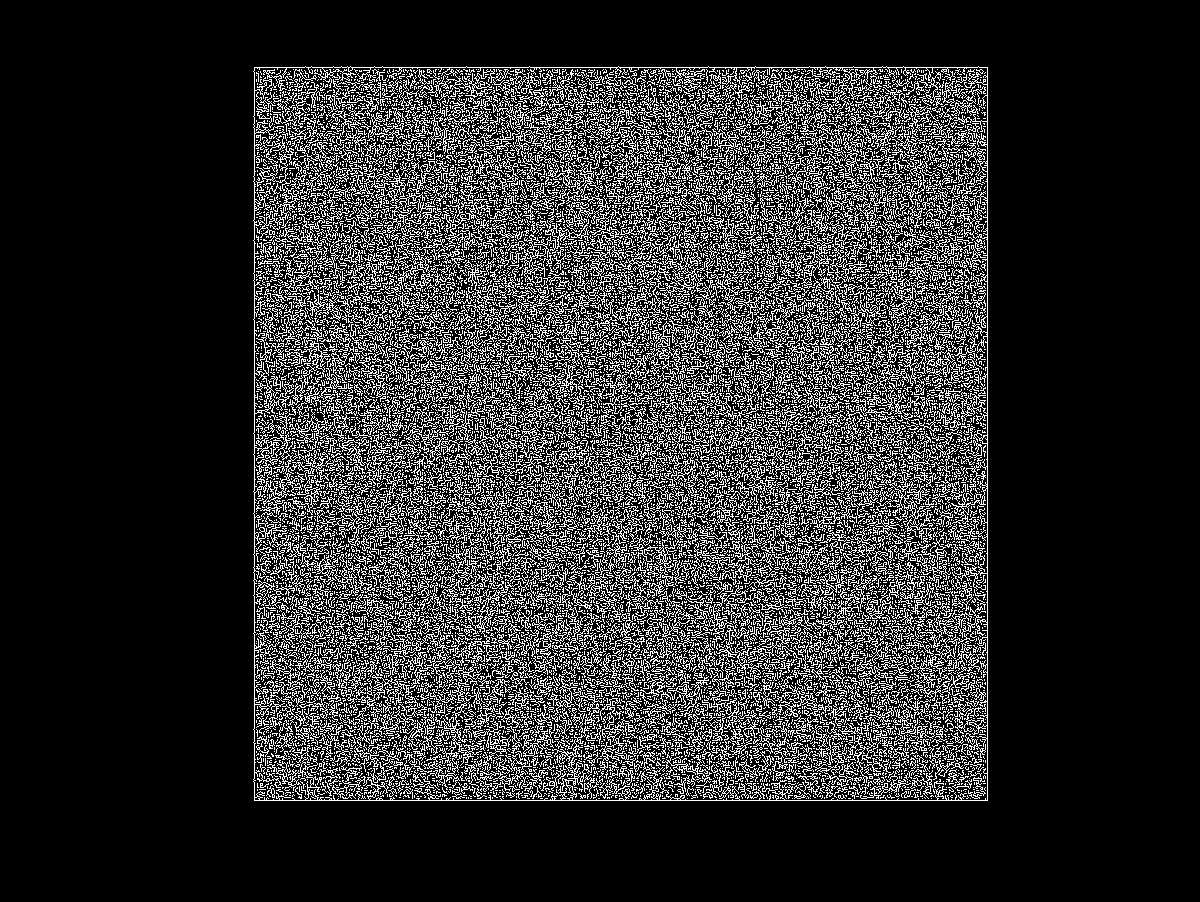
\includegraphics[width=\linewidth]{canny_Eq_Phantom_0p700_4_1_1.jpg}
%  \caption{Canny}\label{fig:awesome_image3}
\endminipage\hfill
\minipage{0.20\textwidth}%
  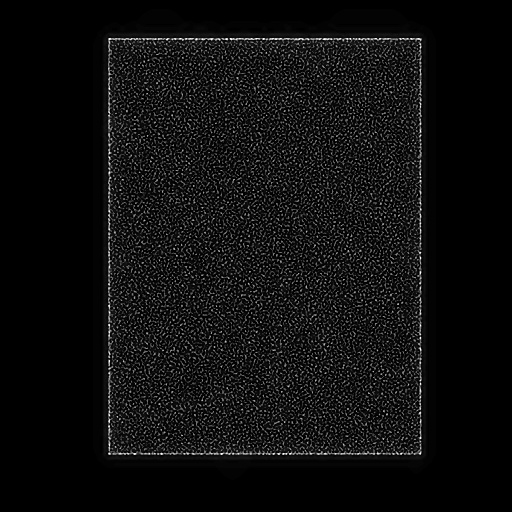
\includegraphics[width=\linewidth]{mult_Eq_Phantom_0p700_4_1_1.jpg}
%  \caption{Multigrid (Piramidal)}\label{fig:awesome_image3}
\endminipage
\caption{Phanton-Sobel-Laplaciano-Canny-Multgrid}\label{fig:awesome_image3}
\end{figure}
Nesta seção serão mostradas imagens com os resultados dos métodos propostos acima. 

Na figura (2) a imagem da maçã foi definida com inserção de ruído aleatório. Isto foi feito para termos uma ideia de como os métodos atuam na detecção de borda e no tratamento dos ruídos. A imagem serviu de teste para todos os operadores definidos acima.

Os resultados dos operadores propostos no artigo bem como os métodos estabelecidos na literatura da área, como: o Sobel, LoG, e LoG Piramidal são mostrados nas figuras (3) a (7), nas quais pode-se notar um bom desempenho, tanto na detecção da borda, como na atenuação de ruídos.


Na figura (6) é mostrado o desempenho do Operador Laplaciano Multigrid (OLM). Podemos observar que a borda apresenta duplicidade e o ruído foi pouco atenuado. Investigando o (OLM), com cuidado, notamos que a duplicidade e o ruído surgiam na interpolação e aplicação do LoG, depois de chegarmos a imagem de referência, isto é,  quando alcançamos a resolução de imagem pré-definida e começamos o processo de interpolação.

Depois de realizado a análise propomos a ideia de suprimir a aplicação do operador $LoG$ no processo de interpolação. Por este motivo definimos o Operador Laplaciano Multigrid Modificado (OLMM), cujo o resultado da aplicação do operador (OLMM) está na figura (7).

Podemos notar que a borda foi detectada de maneira consistente e obtivemos uma forte atenuação do ruído em comparação com os outros métodos.

Com intuito de analisar melhor o potencial do (OLMM) outros testes foram realizados utilizando a imagem da maçã e uma nova imagem de um tabuleiro de xadrez sem ruído, correspondentes às figuras (8) e (12). Nesta parte da pesquisa as comparações se restringiram aos operadores $LoG$ Piramidal e (OLMM).

Nas figuras (9) e (13) foi realizado a diferença entre as imagens finais da aplicação dos dois métodos. Notamos e era esperado, pela observação das figuras (5) e (7), que a borda e o ruído continuaram na imagem comprovado pela existência de uma diferença de nitidez. Este fato nos motivou a aplicarmos a diferença entre os resultados dos dois operadores com as imagens originais sem ruído.

Os resultados são mostrados nas figuras (10) e (11) para a imagem da maçã e (14) e (15) para a imagem do tabuleiro de xadrez. Com as imagens das figuras (10) e (11) podemos notar que a borda está melhor delimitada no método (OLMM) e praticamente não observamos ruído. Comparando ao $LoG$ Piramidal podemos afirmar que o operador (OLMM) tem a borda menos borrada e melhor atenuação dos ruídos.      
 
Nas figuras (14) e (15) podemos confirmar o quanto as bordas estão melhor delimitadas no (OLMM). Podemos ver na figura (15) que entre as casas do tabuleiro de xadrez não tem nenhum espaçamento, diferente do que acontece na figura (14). Devido a este fato podemos afirmar que a detecção de borda com o (OLMM) mantém melhor acurácia em relação a imagem original. 

Os desempenhos dos métodos estão registrados na tabela $(I)$, cada método foi rodado $10$ vezes e realizado a média aritimética para minimizar o efeito da concorrência de processos administrados pelo sistema operacional. Na primeira coluna da tabela temos  os métodos descritos no artigo, na segunda coluna está registrado a média citada acima, a terceira coluna mostra a razão entre os tempos de processamento de cada método ($tm$) e o tempo do método mais rápido, que chamamos de tempo de referência ($tr$), isto é, $Taxa=\frac{tm}{tr}$, na última e quarta coluna está porcentagem de tempo que cada método ficou acima do tempo de referência.    
\begin{table}[h]
\centering
\caption{Tabela de tempo para os métodos propostos}.
\begin{tabular}{|c|c|c|c|}
\hline                  
Método & Tempo & Taxa  & Tempo($\%$) \\
\hline                  
Sobel   & 0.0541s  &  $1.05tr$& $5\%$   \\
LoG     & 0.0513s  &  $tr$& $*$   \\
Log Pir & 0.0600s  &  $1.16tr$& $16\%$ \\
OLM     & 0.0622s  &  $1.21tr$& $21\%$ \\
OLMM    & 0.0564s  &  $1.09tr$& $9\%$    \\ 
\hline                  
\end{tabular}
\end{table}

A figura (1) mostra um gráfico de barras no qual os eixos das abicissas estão posicionados os métodos ($1\textsuperscript{\underline{o}}$ coluna da tabela) e no eixo das ordenadas o tempo de cada método ($2\textsuperscript{\underline{o}}$ coluna da tabela) como explicado acima, e ainda, no topo de cada barra está a razão (Taxa - $3\textsuperscript{\underline{o}}$ coluna da tabela ) entre os tempos.

Os dados apresentados mostram que o operador laplaciano multigrid modificado (OLMM) processou em tempo competitivo com os demais métodos, mesmo utilizando operadores de restrição e interpolação. Esses fatos mostram que a configuração dos métodos tipo Multigrid podem ser eficiênte e ter bom desempenho na detecção de bordas. 

\begin{figure}[!htb]
\centering
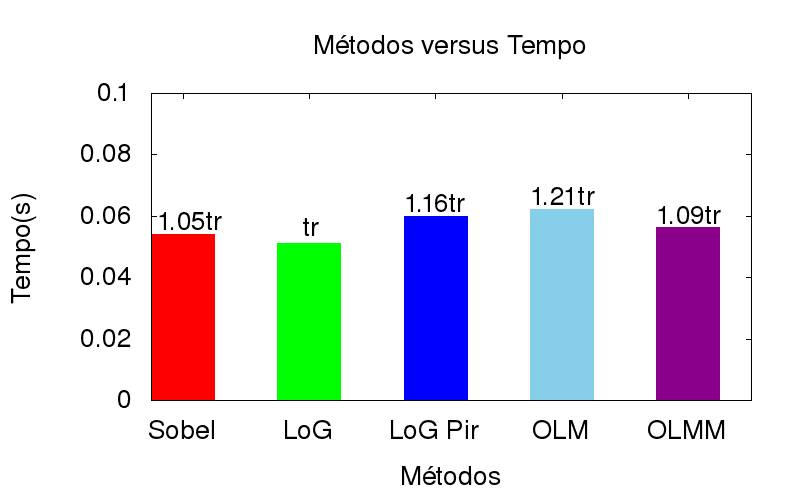
\includegraphics[width=3.0in]{output.jpg}
\label{output}
\caption{Gráfico Métodos versus Tempo.}
\end{figure}


\section{Conclusão}

Neste artigo foram propostos dois operadores de detecção de borda que se chamam respectivamente Operador Laplaciano Multigrid (OLM) e Operador Laplaciano Multigrid Modificado (OLMM).

Com base nas análises das imagens e no desempenho computacional podemos afirmar que o método (OLMM) é competitivo em relação à outros métodos investigados neste artigo estabelecidos na literatura da área. O método mostra uma melhor redução de ruídos bem como um tempo de processamento competitivo com  os outros métodos estudados no artigo. 

Os resultados até aqui alcançados são animadores, pois os métodos Multigrid apresentam um ferramental para otimizar a solução de equações difusivas anisotrópicas que não foram aplicados neste artigo e podem contribuir muito para diminuir ainda mais os ruídos que persistem nas imagens.

Sendo assim, como futuras pesquisas podemos incorporar as ferramentas dos métodos Multigrid para tratamento da anisotropia no operador (OLMM) e investigar outros métodos da visão computacional para detecção de borda, como por exemplo, a representação de imagens no espaço-escala (scale-space representation of an image). 
\bibliographystyle{unsrt}
\bibliography{../bibliografia}
\end{document}
